%UNDERSTANDING DIVISION - WORKSHEET 0 (IN-CLASS INSTRUCTION)
\documentclass[12pt, letterpaper, fleqn]{article}

% ----------------------------------------------------------
% PACKAGES
% ----------------------------------------------------------
\usepackage{graphicx}
\usepackage{xcolor}
\usepackage[most]{tcolorbox}
\usepackage{amsmath, amssymb}
\usepackage{fancyhdr}
\usepackage[utf8]{inputenc}
\usepackage[T1]{fontenc}
\usepackage{enumitem}
\usepackage{geometry}
\usepackage{tikz}
\usepackage{needspace}
\usepackage{multicol}

\usetikzlibrary{arrows.meta, calc, shapes.geometric}

% ----------------------------------------------------------
% PAGE SETUP
% ----------------------------------------------------------
\usepackage{times}
\geometry{letterpaper, top=1.25in, bottom=1.25in, marginpar=0.5in}

% ----------------------------------------------------------
% HEADER / FOOTER
% ----------------------------------------------------------
\newcommand{\logowidth}{3cm}
\setlength{\headheight}{20pt}
\setlength{\footskip}{40pt}

\pagestyle{fancy}
\fancyhf{}
\fancyhead[C]{\small\bfseries Understanding Division}
\fancyfoot[L]{\raisebox{2pt}{
\includegraphics[width=\logowidth]{../kss.png}}}
\fancyfoot[C]{\thepage}
\fancyfoot[R]{3.4.0}

\renewcommand{\footrulewidth}{0.2pt}

% ----------------------------------------------------------
% THEME COLOR
% ----------------------------------------------------------
\definecolor{customteal}{HTML}{2fbdb9}

% ----------------------------------------------------------
% HELPER MACROS
% ----------------------------------------------------------
\newcommand{\blank}{\underline{\hspace{2.2cm}}}
\newcommand{\blanklong}{\underline{\hspace{6.5cm}}}
\newcommand{\blankshorter}{\underline{\hspace{1.5cm}}}

% ----------------------------------------------------------
% DOCUMENT
% ----------------------------------------------------------
\begin{document}

\textbf{Name:} \underline{\hspace{5cm}}
\hfill
\textbf{Date:} \underline{\hspace{3cm}}\\

\begin{tcolorbox}[colback=customteal!20]
    \large\textcolor{black}{\textbf{What is Division?}}
\end{tcolorbox}

\vspace{3mm}
\noindent
Division means **sharing equally** or splitting a group into equal parts.
If you have **6 cookies** and want to share them equally with **2 friends**, you give each friend **3 cookies**.
\[
6 \div 2 = 3
\]

\begin{tcolorbox}[colback=white, colframe=black!25, boxrule=0.6pt, arc=4mm]
\textbf{Visual Representation: Division}
\begin{center}
\begin{tikzpicture}[scale=0.8]
\draw[thick, fill=customteal!10] (0,0) circle (1.1);
\draw[thick, fill=customteal!10] (3.5,0) circle (1.1);
\fill[orange] (-0.3,0.3) circle (0.15); \fill[orange] (0.3,-0.3) circle (0.15); \fill[orange] (0,0) circle (0.15);
\fill[orange] (3.2,0.3) circle (0.15); \fill[orange] (3.8,-0.3) circle (0.15); \fill[orange] (3.5,0) circle (0.15);
\node at (0, -1.4) {Friend 1 (3)};
\node at (3.5, -1.4) {Friend 2 (3)};
\end{tikzpicture}
\end{center}
\end{tcolorbox}

\newpage
\begin{tcolorbox}[colback=customteal!20]
    \large\textcolor{black}{\textbf{Guided Practice: Sharing Equally}}
\end{tcolorbox}

\vspace{5mm}
\begin{enumerate}[itemsep=3cm, leftmargin=0.6cm]
\item Share 8 apples equally among 4 horses. Draw dots in each box to find how many apples each horse gets.
\begin{center}
\begin{tikzpicture}
\draw[thick] (0,0) rectangle (1.2,1.2);
\draw[thick] (2,0) rectangle (3.2,1.2);
\draw[thick] (4,0) rectangle (5.2,1.2);
\draw[thick] (6,0) rectangle (7.2,1.2);
\end{tikzpicture}
\end{center}
Equation: $8 \div 4 =$ \blank

\item Split 15 balloons into 3 equal groups. How many balloons are in each group?
\\
Equation: $15 \div 3 =$ \blank
\end{enumerate}

\end{document}
